%\documentclass[t,handout]{beamer}
\documentclass{beamer}


\usepackage[utf8]{inputenc}
\usepackage[english]{babel}
%\usepackage[tight]{subfigure}
\usepackage{graphicx}
\usepackage{color}
\usepackage{url}
% \usepackage{listings}
%\usepackage[alf]{abntcite}


%\usetheme{Frankfurt} %LEGAL     !!!
% \usetheme{Madrid}     %LEGAL/L%IMPO/COM CAIXA     (sem barra de desenvolvimento)

% \usetheme{Antibes} %NAO
%\usetheme{Berlin} %PODE SER...     (BARRA DE DESENVOLVIMANTO)
% \usetheme{Berkeley}     %FEIO
% \usetheme{Boadilla} %TUDO BRANCO...
% \usetheme{Copenhagen}     %NAO
% \usetheme{Darmstadt} %LEGAL!     !!!
 \usetheme{Dresden}     %LEGAL/LIMPO/SEM CAIXA     (sem caixa fica ruim...)

% \usetheme{Goettingen}     %FEIO DEMAIS!
%\usetheme{Ilmenau} %LEGAL (forte candidato)
% \usetheme{JuanLesPins} %BACANA
% \usetheme{Luebeck}     %FEIO

% \usetheme{Malmoe}     %FEIO
% \usetheme{Warsaw} %NAO...
% \usetheme{Seattle}
% \usetheme{CambridgeUS}
% \usetheme{Singapore}

% \usecolortheme[RGB={130,35,150}]{structure}
% \usecolortheme[RGB={33,33,94}]{structure}
\usecolortheme[RGB={134,153,188}]{structure}
\setbeamertemplate{footline}[frame number]
\setbeamertemplate{navigation symbols}{}

%Hide subsections on teable of contents
%\hypersetup{bookmarksopen=true,bookmarksopenlevel=4}
%\setcounter{tocdepth}{2}



\author[]{\textbf{Leonardo Medeiros}, Hyggo Almeida, Leandro da Silva, Mirko Perkusich and Robert Fischer}

%\date{\today}
\date{20/06/2016}
\institute[]{Federal University Of Campina Grande - BRAZIL
}
\title{A Gait Analysis Approach to Track Parkinson's Disease Evolution Using Principal Component Analysis}
%\logo{\includegraphics[width=0.2\linewidth]{img/logo.png}}
\subtitle{\textbf{CBMS 2016}}

\begin{document}

\begin{frame}
  \titlepage
\end{frame}

% \section{Roteiro}
% \AtBeginSection[]
{\frame{
\frametitle{Summary}
%\tableofcontents
\tableofcontents
}
}






\section{Motivation}
\subsection{}
\begin{frame}{Gait Analysis to Track Parkinson's Disease Evolution}
	\begin{block}{}
	Gait analysis has been strongly applied to evaluate the evolution of neurological diseases such as Parkinson's Disease (PD), which affects about 2$\%$\ of the world population.
	\end{block}

  \begin{block}{}
	In this work, we present a \textbf{reproducible gait analysis to track Parkinson's Disease evolution} by monitoring walking abnormalities. 
  \end{block} 
\end{frame}

\begin{frame}{Gait Analysis}
  \begin{block}{}
  Gait analysis is the systematic study of human locomotion, including qualitative and quantitative assessment.
  \end{block}  
	
	\begin{block}{}
	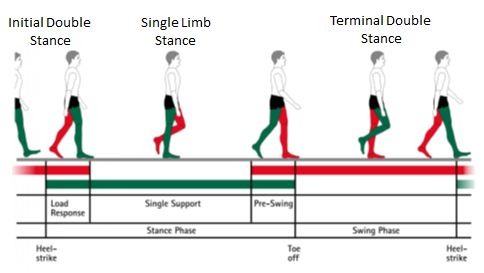
\includegraphics[height=2.2 in]{img/gait-chart.jpg}
	\end{block}
\end{frame}

\begin{frame}{Gait Analysis}
  \begin{block}{}
The human gait is a periodic movement of the limbs during locomotion over a solid substrate. Each gait cycle starts when a foot initiates contact (i.e., heel strike) with the ground and restarts when it touches the ground again.
	\end{block}
\end{frame}

\begin{frame}{Sensors To Acquire VGRF}
  \begin{block}{}
Nowadays, an effective approach is using foot sensors to collect gait data from the forces between the foot and the ground defined as Vertical Ground Reaction Force (VGRF)
  \end{block}
\end{frame}

\begin{frame}{Gait Analysis through VGRF}
  \begin{block}{}
Gait analysis studies the forces and moments of the movement of body segments in a human gait, including the measurement of VGRF. The patients use adapted force sensors under the feet and attached to the shoes to measure the VGRF.
	\end{block}
\end{frame}

\begin{frame}{Motivation}
\begin{block}{}
	Physicians and physiotherapists apply gait analysis \textbf{subjectively in clinical evaluation}, which sometimes is followed by a survey regarding gait quality. This research area has attracted the interest of \textbf{multidisciplinary researchers}.
	\end{block}
\end{frame}

\begin{frame}{PCA for Gait Analysis}
  \begin{block}{}
In this paper, we propose a gait analysis approach to \textbf{track PD evolution by monitoring walking abnormalities}. We \textbf{applied PCA into gait data to detect abnormalities that may indicate the progression of PD}.
  \end{block}
\end{frame}

\begin{frame}{Data Collection}
	\begin{block}{}
	We validated our approach with a public database of foot sensor data, which includes vertical ground reaction force records of healthy subjects and PD patients.
	\end{block}
\end{frame}


\section{PCA for Gait Analysis}
\subsection{}
\begin{frame}{How We Detected Gait Abnormalities ?}
	\begin{block}{}
	We used Principal Component Analysis to identify the gait variance.
	\end{block}
\end{frame}


\begin{frame}{Principal Component Analysis}
	\begin{block}{}
	PCA is a statistic procedure to reduce data and eliminate redundancies. It identifies the data variance and applies linear data transformation to detect the most relevant data components on the first dimension, called the main axis.  The second remaining variance is the secondary axis and so on.
	\end{block}
\end{frame}

\begin{frame}{PCA Step by Step}
	\begin{block}{}
	PCA consists of the following steps: 
		\begin{enumerate}[<+->]
				 \item Scale the measurement data into an \textit{m} x \textit{n} matrix, where \textit{m} is the number of measurement types and \textit{n} is the number of samples;
				 \item Subtract the mean for each measurement type;
				 \item Calculate the \textit{eigenvectors} and \textit{eigenvalues} of the covariance matrix.
				 \item The Calculated \textit{eigenvectors} and \textit{eigenvalues} can be used to project the data into a new space called \textit{eigenspace}.
		\end{enumerate}
	\end{block}
\end{frame}

\begin{frame}{System Overview}
		 \begin{block}{}
			\begin{center}
				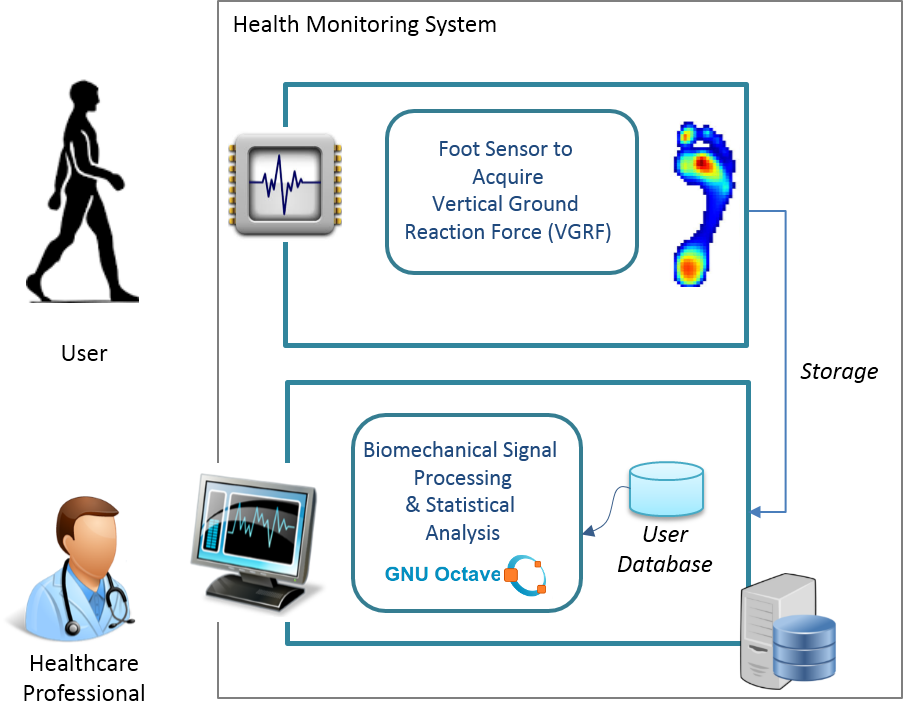
\includegraphics[height=2.2 in]{img/systemoverview.png}
			\end{center}
		 \end{block}
\end{frame}


\begin{frame}{Mean Vector}
		 \begin{block}{}
			\begin{center}
				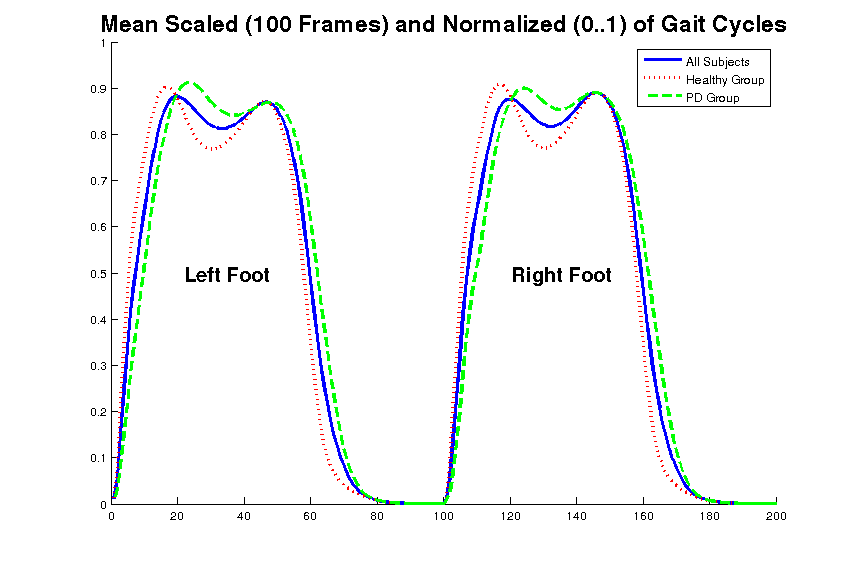
\includegraphics[height=2.2 in]{img/meangait.png}
			\end{center}
		 \end{block}		
\end{frame}

\section{Developed Approach}
\subsection{}
\begin{frame}{Developed Approach}
	\begin{block}{}
	To automate the identification of each gait phase in the VGRF data, it is necessary to use \textbf{signal processing techniques}. 
	\end{block}
	
	\begin{block}{}
	In this work, we focus on the VGRF of each foot and identifying when the foot initiates contact (i.e., start of stance phase) with the ground and when it is off the ground. For this purpose, \textbf{we used the peaks and valleys technique} to identify the beginning and end of each gait cycle.
	\end{block}
\end{frame}

\begin{frame}{Peaks and Valleys}
	\begin{block}{}
		\begin{center}
				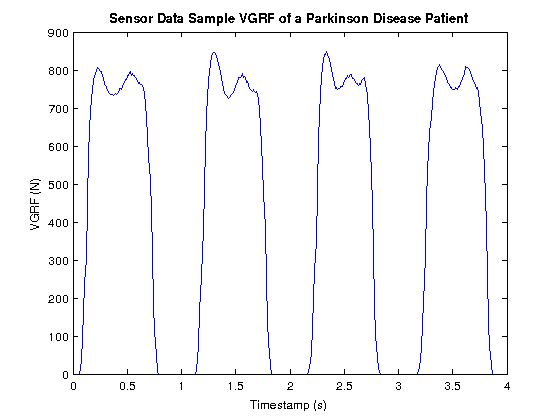
\includegraphics[height=2.2 in]{img/sampleRawData.png}
		\end{center}
	\end{block}
\end{frame}


%\begin{frame}{Biomechanical signal processing}
	%\begin{block}{}
		%\begin{center}
				%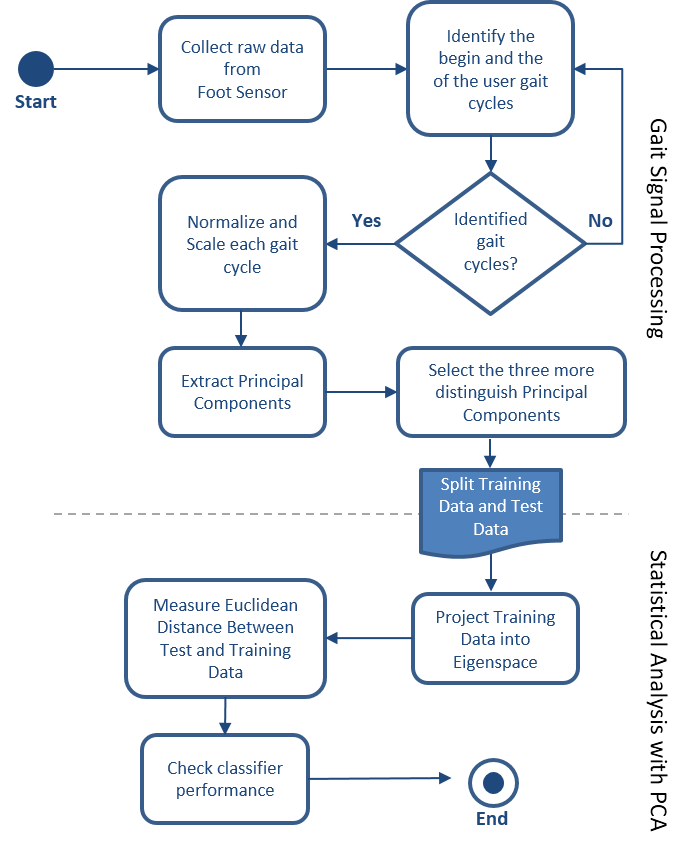
\includegraphics[height=2.2 in]{img/biomecanicalsignal.png}
		%\end{center}
	%\end{block}
%\end{frame}

\begin{frame}{Data Collection}
	\begin{block}{}
	In this work, we used an database under ODC Public Domain Dedication and License. Available at~\textbf{physionet}, which contains the VGRF records of subjects as they walked at their usual pace for approximately 2 minutes on level ground. 
	\end{block}
\end{frame}

\section{Validation}
\subsection{}
\begin{frame}{PCA for Gait Analysis Data Classification}
	\begin{block}{}
		\begin{itemize}[<+->]
			\item PCA defines an orthogonal linear transformation that transforms data into a new coordinate system in which the greatest variance by any projection of data;
			\item We project this data creating a new space;
			\item So, we used the euclidean distance of the test data to the training data to classify each subject as \textbf{PD's Group or Control Group}.
		\end{itemize}
	\end{block}
\end{frame}


\begin{frame}{Projection of PD's (RED) and HEALTHY (BLUE dots)}
	\begin{block}{}
		\begin{center}
				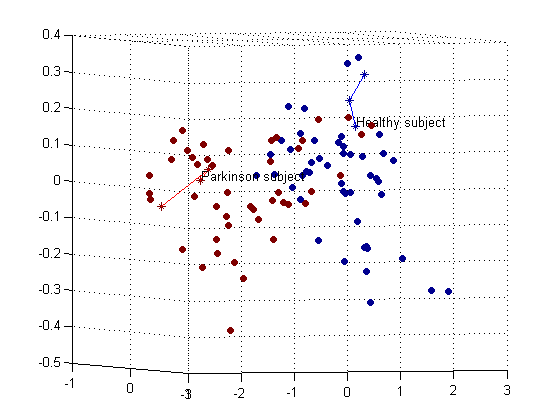
\includegraphics[height=2.6 in]{img/pca-projection-health-parkinson.png}
		\end{center}
	\end{block}
\end{frame}

\begin{frame}{PCA with Euclidean Distance Classifier Performance}
   \begin{block}{}
   
   \begin{columns}[c]
     \begin{column}{0.5\linewidth}
				\begin{table}[!htbp]
					\centering
					\begin{tabular}{l|c|c|}
					\cline{2-3}
					\multicolumn{1}{c}{}                         & \multicolumn{2}{|c|}{\textit{\textbf{Predictive Class}}} \\ \cline{2-3} 
																											 & \textbf{Parkinson}      & \textbf{Control}         \\ \hline
					\multicolumn{1}{|l|}{\textbf{Parkinson}} & 43       & 7           \\ \hline
					\multicolumn{1}{|l|}{\textbf{Control}}     & 12           & 38     \\ \hline
					\end{tabular}
			\end{table}

     \end{column}

     \begin{column}{0.55\linewidth}
						\begin{table}[htbp!]
						\begin{tabular}{|l|r|}
						\hline
						\multicolumn{2}{|l|}{\textbf{Classifier Metrics}} \\ \hline
							\textbf{TpRate}                    & 86.00$\%$\                 \\ \hline
							\textbf{FpRate}                    & 24.00$\%$\                \\ \hline
							\textbf{Precision}                 & 78.18$\%$\                \\ \hline
							\textbf{Accuracy}                  & 81.00$\%$\                \\ \hline
							\textbf{F-Score}                 & 81.90$\%$\                \\ \hline
						\end{tabular}
						\end{table}
    \end{column}
\end{columns}
\end{block}
\end{frame}


\section{Questions}
\begin{frame}{Questions}
	\begin{block}{Reproducible Research}
	Our source code is under GPL License Version 3.0 and can be reproduced using an Open Source Application for numerical computations (Octave Version 3.8.1). 
	\end{block}

	\begin{block}{Source Code and Relevant Data}
	To reproduce our results we created a web page containing all the relevant information~\url{http://gaitparkinson.wordpress.com}. 
	\end{block}
\end{frame}

\bibliographystyle{IEEEtran}
\bibliography{sigproc2,IEEEFormat}

\end{document}
	